%
%  This is an example of how a LaTeX thesis should be formatted.  This
%  document contains chapter 1 of the thesis.
%
%  Time-stamp: "[sample-chapter1.tex] last modified by Scott Budge (scott) on 2017-01-12 (Thursday, 12 January 2017) at 10:20:50 on goga.ece.usu.edu"
%
%  Info: $Id: sample-chapter1.tex 998 2017-03-21 16:44:33Z scott $   USU
%  Revision: $Rev: 998 $
% $LastChangedDate: 2017-03-21 10:44:33 -0600 (Tue, 21 Mar 2017) $
% $LastChangedBy: scott $
%

\chapter{INTRODUCTION}
%%%%%%%% This line gets rid of page number on first page of text
\thispagestyle{empty}
%%%%%%%%%%%%%

Image compression or image coding is the process of reducing the
redundancy in the image data that may result in some loss of
information.  Vector quantization (VQ)\footnote{The acronym VQ is used
  as an abbreviation for both vector quantization and vector
  quantizer.} is one such technique.

\section{Background}
Binary splitting is illustrated in Fig.~\ref{fig:split}.

\begin{figure}[htbp]
\centering
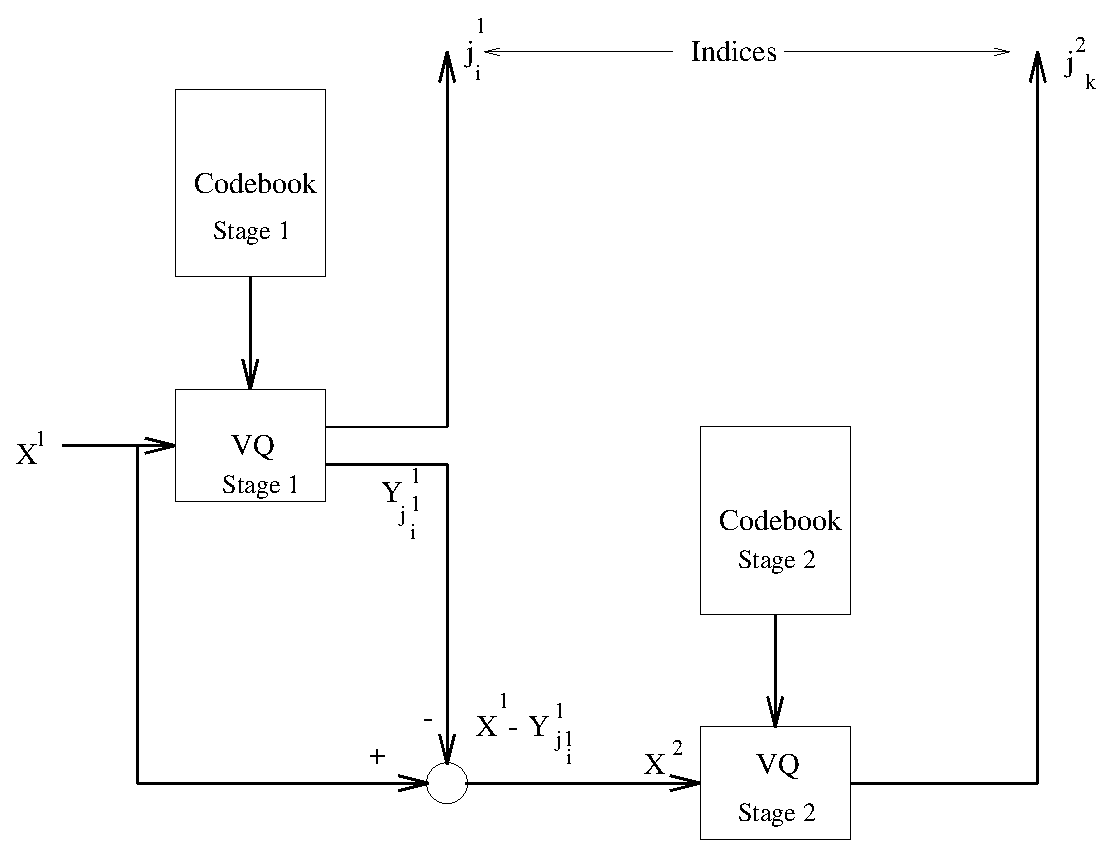
\includegraphics[width=0.7\textwidth]{samplefig}
\caption{Binary splitting.}
\label{fig:split}
\end{figure}
This figure is generated using an open-source figure drawing package
(called {\tt fig}).  Any figure drawing package can be used to
generate figures.  The easiest format for output is to output the
figures in {\tt .pdf} format for inclusion in the {\tt .tex} file.

% For the following three examples, note the problems with the xdvi
% viewer described in the thesis.tex and the README.txt files.

%%%%%%%%%%%%%%%%%%%%%%%%%%%%%%%%%%%%%%%%%%%%%%%%%%%%%%%%%%%%%%%%%%
% TikZ example:  This is the same as the above figure, except done
% using TikZ.
%%%%%%%%%%%%%%%%%%%%%%%%%%%%%%%%%%%%%%%%%%%%%%%%%%%%%%%%%%%%%%%%%%
\begin{figure}[!t]
	\begin{center}
		\begin{tikzpicture}[every text node part/.style={align=center}]
			% Place nodes:
			\draw (0,0) node[draw] (book1) {{\em Codebook}\\ {\small Stage 1}};
			\draw ($(book1) + (0,-2)$) node[draw] (vq1) {{\em VQ}\\ {\small Stage 1}};
			\draw ($(vq1) + (3,-3)$) node[circle,draw,minimum height=1cm] (adder) {$\Sigma$};
			\draw ($(adder) + (5,0)$) node[draw] (vq2) {{\em VQ}\\ {\small Stage 2}};
			\draw ($(vq2) + (0,2)$) node[draw] (book2) {{\em Codebook}\\ {\small Stage 2}};
			
			% Draw arrows:
			\draw [-latex] (book1.south) -- (vq1.north);
			\draw [-latex] (book2.south) -- (vq2.north);
			\draw [-latex] ($(vq1.north east)+(0,-.25)$) node(vqout1) {} -| ($(adder.north)+(0,6)$) node[anchor=south west] (ji) {$j_i$};
			\draw [-latex] ($(vq1.south east)+(0,.25)$) node(vqout2) {} -| (adder.north);
			\draw [-latex] (vq1.west) -- ($(vq1.west)+(-1,0)$) node (in) {} |- (adder.west);
			\draw [-latex] (vq2.east) -| ($(ji.south west) + (7,0)$) node[anchor=south west] (jk2) {$j_k^2$};
			\draw ($(vq1.west)+(-2,0)$) node[anchor=east] {$X^1$} to[short,o-*] (in);
			\draw [-latex] (in) -- (vq1.west);
			\draw [-latex] (adder.east) -- (vq2.west);
			
			% Draw remaining labels:
			\draw (vqout2) node[anchor=north west] {$Y_{j_i^1}^1$};
			\draw (adder.north) node[anchor=south east] {$-$};
			\draw (adder.west) node[anchor=south east] {$+$};
			\draw (adder.east) node[anchor=south west] {$X^1-Y_{j_i^1}^1$};
			\draw (vq2.west) node[anchor=south east] {$X^2$};
			
			% Draw annotation:
			\draw ($(ji)!0.5!(jk2) + (0,1)$) node (indices) {\Large Indices};
			\draw[thick,-triangle 45] (indices.west) to [out=180,in=45] (ji.north east);
			\draw[thick,-triangle 45] (indices.east) to [out=0,in=135] (jk2.north west);
		\end{tikzpicture}
		\caption{Binary splitting (drawn with TikZ).}
		\label{fig:split_tikz}
	\end{center}
\end{figure}

%%%%%%%%%%%%%%%%%
% CircuiTikZ example:
%%%%%%%%%%%%%%%%%
\begin{figure}[!t]
	\begin{center}
		\begin{tikzpicture}
			\draw (0,0) node[op amp,scale=0.75] (oa){};
			\draw (oa.out) to[short, -*] ++(1,0) node (n1) {};
			\draw (n1.base) -- ++(1,0) to[C,l^=$C_S$,v_=$V_{\textrm{\small out,ofs}}$] ++(3,0) 	node[anchor=west] (n4) {$V_{\textrm{\small out}}$};
			\draw (oa.-) to[short,-*] ++(-1,0) node (n2) {};
			\draw (n2.base) |- ++(1,2) to[C] ++(2,0) -| (n1.base);
			\draw ($(oa.+)+(0,-3)$) node[ground] {}  to[vsource=$V_{\textrm{\small in,ofs}}$] (oa.+);
			\draw (n2.base) to[C] ++(-2,0) node[anchor=east] (n3) {$V_{\textrm{\small in}}$};
		\end{tikzpicture}
		\caption{Circuit example drawn using circuitikz.}
		\label{fig:circuitikz_exmple}
	\end{center}
\end{figure}

There are many other ways to create figures.  One package compatible
with \LaTeX\ is TikZ.  An example is given in
Fig.~\ref{fig:split_tikz}. This is identical to Fig.~\ref{fig:split},
except that it is done within the compiling process of \LaTeX.
Another example of a third-party figure package is given in
Fig.~\ref{fig:circuitikz_exmple}.  This circuit was generated using
the {\tt circuitikz} package.

It is important that there is no text between figures when they are
referenced close together in the text.  They should be ``stacked''
without text in between as seen above.

A final way of creating graphs is to use a open-sourse package called
{\tt PGFPlots}.  An example of a good-looking graph generated using
this package is given in Fig~\ref{fig:pgfplots_example}.  Note that
this figure is large enough that it is pushed by \LaTeX\ to another
page by itself and nicely centered.
%%%%%%%%%%%%%%%%%
% PGFplots example:
%%%%%%%%%%%%%%%%%
\begin{figure}[tbh]
\begin{center}
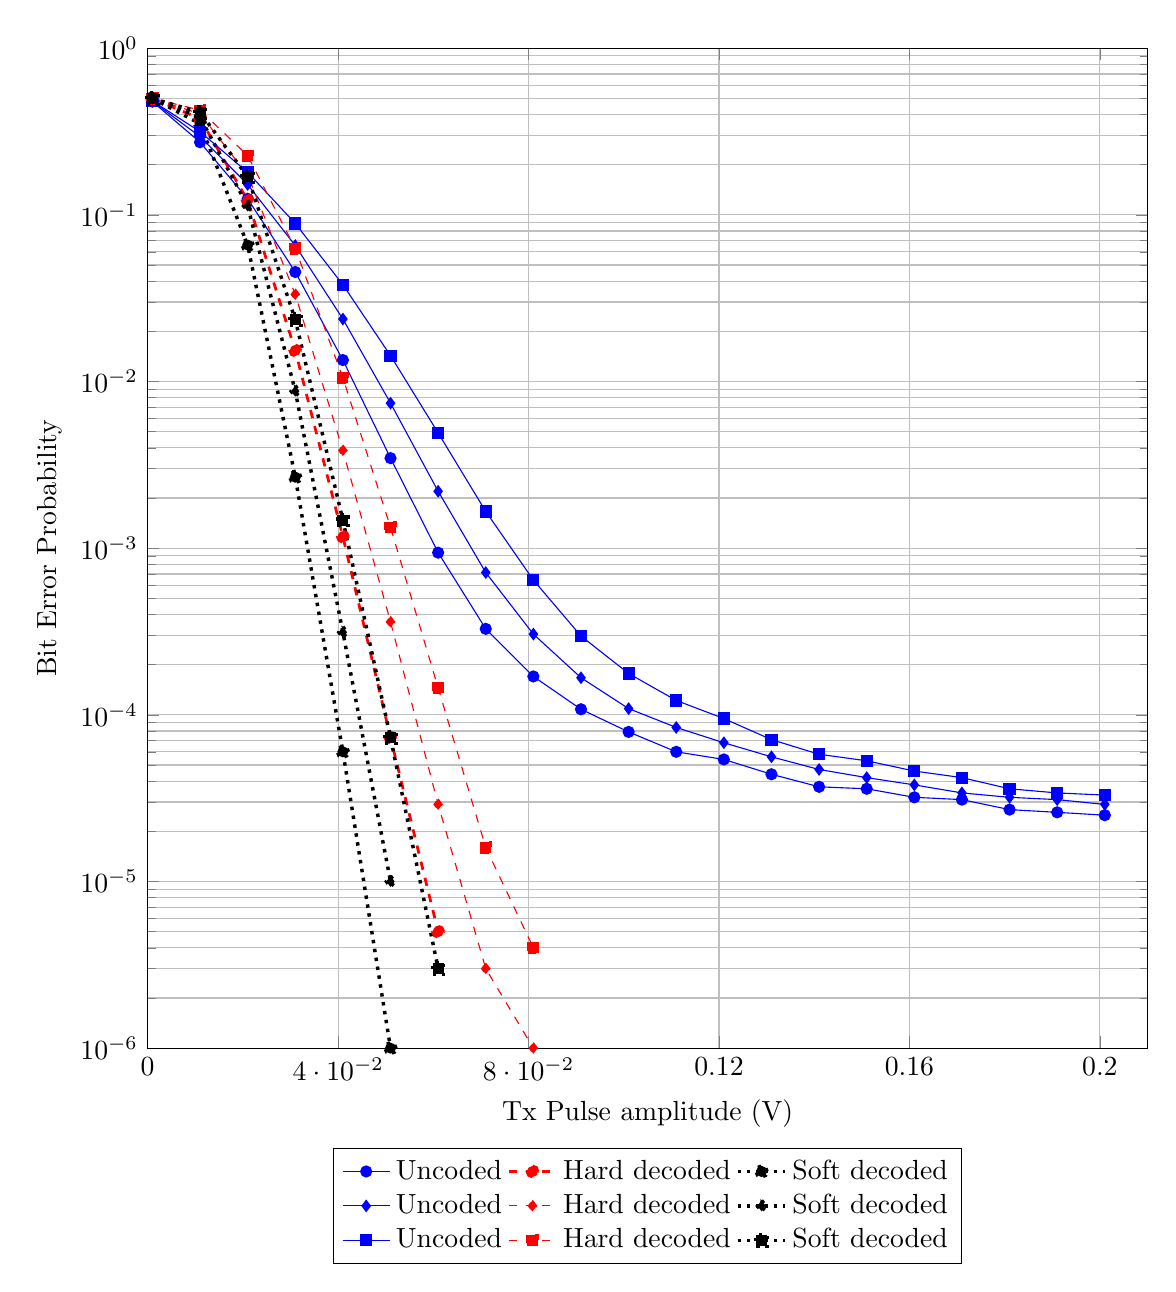
\begin{tikzpicture}
\begin{semilogyaxis}
[% 
scale only axis, 
width=5in, 
height=5in, 
xmin=0, 
xmax=0.21, 
xtick={0, 0.04, ..., 0.2},
ymin=1e-006, 
ymax=1, 
yminorticks=true, 
%xlabel={$\text{Tx Pulse amplitude }(\si{\volt})$},
xlabel={Tx Pulse amplitude (V)},
ylabel={Bit Error Probability}, 
xmajorgrids, 
ymajorgrids, 
yminorgrids,
legend columns=3,
legend style={at={(0.5,-0.1)},anchor=north},%{at={(0.5,-0.5)},anchor=south},
cycle multi list={%
   color list\nextlist
   [3 of]mark list}
]

%%%%%%%%%%%%%%%%%%%%%%%%%%%%%%%%%%%%%%%%%%%%%%%%%%%%%%%%%%%%%%%%%%
%8p_NF4_uncoded
\addplot [ color=blue, solid, mark=*, mark options={fill=blue} ] 
coordinates{  
(0.001,0.478052)(0.011,0.272706)(0.021,0.124776)(0.031,0.045402)(0.041,0.013449)(0.051,0.003469)(0.061,0.00094)(0.071,0.000328)(0.081,0.00017)(0.091,0.000108)(0.101,7.9e-005)(0.111,6e-005)(0.121,5.4e-005)(0.131,4.4e-005)(0.141,3.7e-005)(0.151,3.6e-005)(0.161,3.2e-005)(0.171,3.1e-005)(0.181,2.7e-005)(0.191,2.6e-005)(0.201,2.5e-005)  
    };
\addlegendentry{Uncoded}

%8p_NF4_hard
\addplot [ color=red, line width=1pt,dashed, mark=*,  mark options={fill=red},]
coordinates{  
(0.001,0.499268)(0.011,0.377753)(0.021,0.122226)(0.031,0.01535)(0.041,0.001172)(0.051,7.3e-005)(0.061,5e-006)(0.071,0)  
};
\addlegendentry{Hard decoded}

%8p_NF4_soft
\addplot [ color=black, dotted, line width=1.25pt,mark=*, mark options={fill=black} ] 
coordinates{  (0.001,0.49911)(0.011,0.352208)(0.021,0.065849)(0.031,0.002668)(0.041,6e-005)(0.051,1e-006)  
};
\addlegendentry{Soft decoded}

%%%%%%%%%%%%%%%%%%%%%%%%%%%%%%%%%%%%%%%%%%%%%%%%%%%%%%%%%%%%%%%

%%%%%%%%%%%%%%%%%%%%%%%%%%%%%%%%%%%%%%%%%%%%%%%%%%%%%%%%%%%%%%%%%%
%8p_NF5_uncoded
\addplot [ color=blue, solid, mark=diamond*, mark options={fill=blue} ]
coordinates{  (0.001,0.480507)(0.011,0.294723)(0.021,0.1521)(0.031,0.065413)(0.041,0.023695)(0.051,0.007415)(0.061,0.002195)(0.071,0.000714)(0.081,0.000305)(0.091,0.000167)(0.101,0.000109)(0.111,8.4e-005)(0.121,6.8e-005)(0.131,5.6e-005)(0.141,4.7e-005)(0.151,4.2e-005)(0.161,3.8e-005)(0.171,3.4e-005)(0.181,3.2e-005)(0.191,3.1e-005)(0.201,2.9e-005)      };
\addlegendentry{Uncoded}

%8p_NF5_hard
\addplot [ color=red, dashed, mark=diamond*, mark options={fill=red} ]
coordinates{  (0.001,0.499279)(0.011,0.403647)(0.021,0.17325)(0.031,0.033326)(0.041,0.003852)(0.051,0.000361)(0.061,2.9e-005)(0.071,3e-006)(0.081,1e-006)        
};
\addlegendentry{Hard decoded}

%8p_NF5_soft
\addplot [ color=black, dotted, line width=1.25pt,mark=diamond*, mark options={fill=black} ]
coordinates{  (0.001,0.499265)(0.011,0.385162)(0.021,0.113072)(0.031,0.008749)(0.041,0.000313)(0.051,1e-005)(0.061,0)  
};
\addlegendentry{Soft decoded}
%%%%%%%%%%%%%%%%%%%%%%%%%%%%%%%%%%%%%%%%%%%%%%%%%%%%%%%%%%%%%%%

%%%%%%%%%%%%%%%%%%%%%%%%%%%%%%%%%%%%%%%%%%%%%%%%%%%%%%%%%%%%%%%%%%
%8p_NF6_uncoded
\addplot [ color=blue, solid, mark=square*, mark options={fill=blue} ]
coordinates{  (0.001,0.482503)(0.011,0.315407)(0.021,0.179759)(0.031,0.088806)(0.041,0.038068)(0.051,0.014303)(0.061,0.004914)(0.071,0.001661)(0.081,0.000644)(0.091,0.000297)(0.101,0.000177)(0.111,0.000122)(0.121,9.5e-005)(0.131,7.1e-005)(0.141,5.8e-005)(0.151,5.3e-005)(0.161,4.6e-005)(0.171,4.2e-005)(0.181,3.6e-005)(0.191,3.4e-005)(0.201,3.3e-005)       };
\addlegendentry{Uncoded}

%8p_NF6_hard
\addplot [ color=red, dashed, mark=square*, mark options={fill=red} ]
coordinates{
(0.001,0.499326)(0.011,0.424875)(0.021,0.22663)(0.031,0.062807)(0.041,0.010536)(0.051,0.001333)(0.061,0.000145)(0.071,1.6e-005)(0.081,4e-006)(0.091,0)  
};
\addlegendentry{Hard decoded}

%8p_NF6_soft
\addplot [ color=black, dotted, line width=1.25pt,mark=square*, mark options={fill=black} ] 
coordinates{  (0.001,0.499363)(0.011,0.411563)(0.021,0.169253)(0.031,0.02352)(0.041,0.001472)(0.051,7.3e-005)(0.061,3e-006)(0.071,0)      
};
\addlegendentry{Soft decoded}

%%%%%%%%%%%%%%%%%%%%%%%%%%%%%%%%%%%%%%%%%%%%%%%%%%%%%%%%%%%%%%%

\end{semilogyaxis}

\end{tikzpicture}

\caption{Example figure made with PGFplots. Originally created in Matlab, then exported using the Matlab2TikZ script (available from Matlab Central). Then pasted into the \LaTeX\ document and edited for style. \label{fig:pgfplots_example} }
\end{center}
\end{figure}



% For use with multiple-paper format, uncomment the fillowing:
% \pagebreak
% \bibliographystyle{IEEEtran}
% \bibliography{IEEEabrv,BibFile1}  % uses the references stored in BibFile1.bib for this chapter

% Local Variables:
% TeX-master: "newhead"
% End:
